\chapter{熵与Kullback-Leibler散度}\label{chap:information-theory}

人脑和机器的区别是什么?我们有可能模拟人脑的功能吗?这些问题根植于认知科学和人工智能领域. 在20世纪50年代,计算机科学、认知科学和人工智能仍然处于萌芽状态. 就是在这个时候,基于对人类如何解决问题和决策的研究,Herbert A. Simon提出,人脑其实是一个“信息处理器”,也就是输入信息(视觉、听觉等),进行处理,然后输出信息(动作、语言等). 从这个观点上,人脑和机器并无区别. 

基于这样的观点,Simon和Allen Newell、 J. C. Shaw一起合作,制造了逻辑理论家(Logic Theorist)、通用问题求解器(General Problem Solver,GPS)等计算机程序. 逻辑理论家可以证明《数学原理》(作者是Whitehead和Russell)第二章前52个定理中的38个,而GPS则可以解决汉诺塔问题. 这展现出“信息处理器”观点的巨大潜力. 

时至今日,“信息处理器”的观点已经深入认知科学和人工智能研究者的心中. 然而,信息是一个特别抽象的概念. 它不像重量,可以从沉甸甸的铅块中直观感受到. 那么,信息到底是什么?本章将要讨论这一问题,并给出它在人工智能领域的应用. 

\section{熵}\label{sec:entropy}


\subsection{概念的导出}

我们常说“恐惧来源于未知”,信息似乎代表着某种确定的东西,某种知识,因而和不确定性有相反的关系. 更精确地说,\emph{消除不确定性的东西被称为信息.} 当然,这句话本身似乎是一种循环解释,它既没有回答信息是什么也没有回答不确定性是什么. 所以我们进一步的问题是,给定一个“对象”,如何定量衡量它不确定性(或信息量)?

我们先从一个例子看起. 
\begin{example}[信息论读本]
    假设我们有一个信息论的读本(例如本章就是),我们想要衡量它的信息量. 我们面临的第一个困难是,同样的内容对于不同的人来说,信息量是完全不同的. 已经学过信息论的读者再看这一部分内容,他获得的信息会比没有学过的读者要少得多. 因此,我们很难直接给\emph{单个对象}衡量它的信息量. 

    但是,信息论读本的读者背景是多样的、不确定的,可能学过信息论,可能只学过概率论,也可能什么都没学过. 要衡量这本书的信息量,我们可以考虑所有可能的读者背景,然后给出一个信息的概率分析. 例如,读这本书的读者大概率不是信息论专家,但有一定概率论的背景,他们可以获得很多信息;而还有很少部分读者精通信息论,因此这本书给他们的信息量就很少. 但综合来看,这本书的信息量依然是不少的. 
\end{example}

以上例子说明了这样一种思想:将世界视为不确定的,有多种可能的结果,然后考虑这一堆结果所带来的平均信息量.

我们可以用数学来表述上面的考虑,假如我们进行一次试验,一共有$n$种可能的结果,第$i$种发生的概率为$p_i$. 我们预测试验的结果,如果越能正确地预测,那么就说明我们对这个试验中包含的信息知道的越多. 
\begin{itemize}
    \item 假如$p_1=1$,那么我们完全确定试验一定会产生结果$1$;
    \item 如果$p_i=1/n$,那么我们完全无法预计试验的结果.
\end{itemize}
我们对试验结果的预期与试验结果的概率分布有密切联系. 因此概率分布给我们带来了\emph{信息},使得我们能够产生不同的判断. 另一方面,概率分布带来了\emph{不确定性},使我们不能总是确信预言会成真. 

我们遵循“信息论之父”Shannon的思路,为信息提供一个严格的数学模型:\emph{熵}. 假设随机变量$X$表示了所有可能的结果(编号为$1$到$n$),$\Pr(X=i)=p_i$,$p=(p_1,\dots,p_n)$,有时候也把$p_i$写作$p(i)$. 我们把不确定性度量记为$H(p)$. Shannon假设$H$满足以下三个性质:
\begin{enumerate}
    \item $H$是一个连续函数.
    \item 事件结局可能数变多则不确定性增大:$p_i=1/n$时,$H(p)$随$n$单调递增,$n$是正整数.
    \item 如果一个试验被分成了两个相继的试验,那么原来的$H$应该等于分开之后的$H$的加权和.
\end{enumerate}

前两个假设都比较好理解,我们现在具体解释第三个假设.  
\begin{figure}[ht]
    \centering
    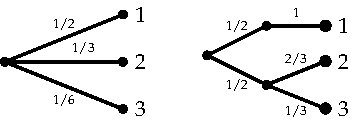
\includegraphics[width=0.6\textwidth]{Figures/information-theory/decomposition-assumption.pdf}
    \caption{Shannon的第三个假设}
    \label{fig:decomposition-assumption}
\end{figure}

如图\Cref{fig:decomposition-assumption} 所示,假设我们有一个试验,有三种可能的结果,$1,2,3$,概率分别为$1/2,1/3,1/6$. 该试验的不确定性是$H(1/2,1/3,1/6)$. 

我们把试验分成两步相继的试验(右图). 第一步试验有两种可能的结果,概率分别都是$1/2$.
\begin{itemize}
    \item  当第一步试验出现上面的结果时,第二步试验以概率$1$产生结果$1$;
    \item  当第二步试验出现下面的结果时,第二步试验以概率$2/3$产生结果$2$,以概率$1/3$产生结果$3$.
\end{itemize}
我们可以看到,分成两步之后,第一步试验的不确定性是$H(1/2,1/2)$,第二步试验的不确定性有一半概率是$H(1)$(上面的分支),有一半概率是$H(2/3,1/3)$(下面的分支),因而加权的不确定性是$1/2\cdot 0+1/2\cdot H(2/3,1/3)$. 因此第三个假设可以具体表述为
\[
H\left(\frac{1}{2},\frac{1}{3},\frac{1}{6}\right)=H\left(\frac{1}{2},\frac{1}{2}\right)+\left[\frac{1}{2}\cdot H(1)+\frac{1}{2}\cdot H\left(\frac{2}{3},\frac{1}{3}\right)\right].
\]

这里,我们可以看出Shannon的哲学思想:不确定性只来自于概率分布而不是具体对象. 他的考虑具有浓厚的工程意味,正如他自己针对通信的数学理论所说:“消息是具有含义的……然而,通信的语义层面并不是工程问题所关心的. ”正是因为抽象掉了具体考虑的对象,信息论的应用才变得如此广泛. 

基于上面三个假设,Shannon证明了如下定理,这一定理直接给出了熵的概念.

\begin{theorem}[Shannon定理]\label{thm:Shannon-thm}
    $H$满足三个假设当且仅当
    \[H(p)=-C\sum_{i}p_i\log p_i,\]
    其中$C$是正常数,$0\log 0=0$.
\end{theorem}
这一定理的证明较长并且和后面的讨论关联较小,所以我们在\Cref{sec:Shannon-thm-proofs}中给出证明.

根据对数的的换底公式,可以将$C\log p_i$写为$\log_bp_i$,这里$C=1/\log b$. 于是,Shannon定理直接给出了熵的如下定义:
\begin{definition}[熵]
    分布列$p=(p_1,\dots,p_n)$的\textbf{熵}定义为
    \[H(p)=-\sum_{i=1}^np_i\log_b p_i.\]
    其中$b=\e$(自然对数底数),$0\log 0=0$. 当$b=2$时,我们记熵为$H_2(p)$.
\end{definition}

通常来说,使用$\e$作为底数会使得数学推导简洁,而用$2$为底数则常常是讨论信息量时的习惯. 在\Cref{sec:entropy-and-communication}中,我们将讨论熵在通信中的含义,以$2$为底的时候熵的实际意义会更清楚些. 如果没有特别强调,我们在讨论时总是假设$b=\e$.

熵的定义还可以用数学期望的形式写出. 假设$X$的分布列是$p$,$p(i)=\Pr(X=i)$,那么我们也可以把熵写成期望的形式:
\[H(p)=-\E[\log p(X)].\]
每一个(离散)随机变量$X$会确定一个分布列$p_X$,因此我们也可以定义随机变量的熵:
\begin{definition}[随机变量的熵]
    随机变量$X$的\textbf{熵}定义为
    \[H(X)=-\E[\log p_X(X)].\]
    其中$p_X$是$X$的分布列,$0\log 0=0$.
\end{definition}

尽管从信息论的角度我们可以唯一确定熵的定义,但是熵的概念在物理学上早就已经存在. 下面我们给出统计力学中熵的推导过程. 

在经典力学中,物理系统的状态由粒子的位置和动量(也就是速度)完全确定,将粒子位置和动量可能的值集合称为\emph{相空间},于是物理系统的演化就是相空间中的粒子状态的变化. 

将相空间等分成$m$个单元,编号$1$到$m$. 假设相空间中有$N$个可区分的粒子,相互独立,没有相互作用,每个粒子等可能出现在每一个单元中. 如果单元$i$中有$N_i$个粒子,那么按照粒子在单元中的分布来看,系统处于某个特定状态的概率为
    \[P=\frac{N!}{N_1!\dots N_m!}\left(\frac1m\right)^N.\]
这是一个多项分布. 两边取对数,得
    \[\log P=\log(N!)-\sum_i\log(N_i!)-N\log m.\]
考虑充分大的$N_i$,由Stirling公式,有
\begin{align*}
    \log(N_i!)\sim\log\left(\sqrt{2\pi N_i}\left(\frac{N_i}{\e}\right)^{N_i}\right)\sim N_i\log N_i.    
\end{align*}
因此,
\begin{equation}
    \log P\sim N\log N-\sum_i N_i\log N_i- N\log m\sim N\log N-\sum_i N_i\log N_i.\label{eq:logP}
\end{equation}
假设$N_i$充分大的时候,$N_i/N$呈现固定的比例$p_i$,那么
    \begin{align*}
        N\log N-\sum_i N_i\log N_i&\sim N\log N-\sum_i Np_i\log(Np_i)\\
        &=-N\sum_i p_i\log p_i.
    \end{align*}
 $\log P\sim -N\sum_i p_i\log p_i$. 于是我们证明了:
    \[\frac1N\log P\to H(p_1,\dots,p_m),\quad N\to\infty.\]
因此,熵刻画了充分多粒子的物理系统某种特定状态出现概率!熵越大的系统越有可能达到. 更进一步,在统计力学中有Boltzmann $H$-定理:孤立的粒子系统会向着熵($H$)增加的方向演化,并最终达到熵最大的状态. $H$-定理是热力学第二定律的微观解释,熵越大的系统出现概率越大、越混乱、越接近均衡.

\subsection{概念与性质}
现在,我们将进一步探讨熵的若干拓展定义,并讨论他们的性质. 

首先,我们考虑最简单的情形,即分布列为$(p_1,p_2)$,此时,我们不妨设$p_1=p$,$p_2=1-p$,那么熵就是
    \[H(p_1,p_2)=H(p,1-p)=-p\log p-(1-p)\log(1-p).\]
$H$是关于$p$的函数,作图如\Cref{fig:entropy-figure} 所示.
\begin{figure}[ht]
        \centering
        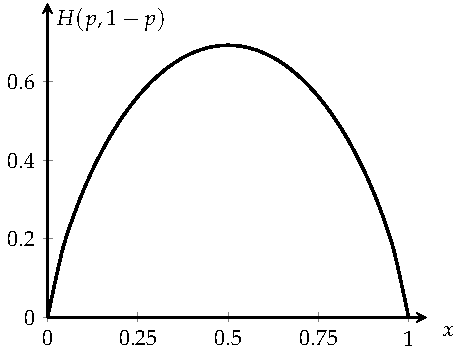
\includegraphics[width=0.6\textwidth]{Figures/information-theory/entropy-figure.pdf}
        \caption{熵$H(p)$的图像.}
        \label{fig:entropy-figure}
\end{figure}

利用导数的方法,很容易证明:
\begin{proposition}\label{prop:entropy-2prob}
    $H(p)$在$p\in (0,1/2)$严格单调递增,在$p\in (1/2,1)$严格单调递减. 它的最小值是$0$,在$p\in\{0,1\}$取得;它的最大值是$\log 2$,在$p=1/2$取得.    
\end{proposition}
\begin{proof}
    我们有
    \[H'(p)=-\log p-1-\log(1-p)+1=\log(p^{-1}-1),\]
    $H'(p)$是一个关于$p$单调递减的函数. 我们有如下分类讨论:
    \begin{itemize}
        \item 当$p\in (0,1/2)$时,$p^{-1}-1>1$,所以$H'(p)>0$,$H(p)$是单调递增的;
        \item 当$p\in (1/2,1)$时,$p^{-1}-1<1$,所以$H'(p)<0$,$H(p)$是单调递减的;
        \item 当$p=1/2$时,$H'(p)=0$,结合前两点,$H(p)$取得最大值. 
    \end{itemize}
    $H(0)=H(1)=0$,$H(1/2)=\log 2$,因此命题得证.
\end{proof}
这与我们对于“不确定性”的直觉是相一致的:当$p$接近$0$或$1$时,我们对于$X$的取值几乎是确定的,因此熵接近$0$;当$p$接近$1/2$时,我们对于$X$的取值几乎是完全不确定的,因此熵接近最大值$\log 2$. 
 
实际上,这样的性质对于一般的分布也是成立的,我们分别将他们写在\Cref{prop:entropy-nonnegative} 和\Cref{prop:entropy-maximum} 中.

考虑一般分布的熵$H(p)=H(p_1,\dots,p_n)$. 我们有如下性质:
\begin{proposition}\label{prop:entropy-nonnegative}
    $H(p)\geq 0$,等号成立当且仅当某个$p_i=1$.
\end{proposition}
\begin{proof}
这是一个典型的证明,主要的技巧是使用熵的期望形式. 考虑随机变量$X$,其分布列为$p$. 回忆Jensen不等式(\Cref{thm:jensen}):如果$f$是一个严格凸函数,那么
\[\E[f(X)]\geq f(\E[X]).\]
等号成立当且仅当$X$是常数.

因为$-\log(\cdot)$是严格凸函数,所以根据Jensen不等式
\[H(X)=\E[-\log p(X)]\geq-\log\E[p(X)]\geq -\log 1=0.\]
等号成立当且仅当$X$是常数,即对某个$i$,$p(i)=1$.
\end{proof}

\begin{proposition}\label{prop:entropy-adjust}
    $p_i$朝着相等方向改变的时候$H$增加. 也就是说,假设
    \[ p_i<p_i'\leq p_j'<p_j,\quad p_i+p_j=p_i'+p_j',\]
    那么,用$p_i'$和$p_j'$代替原来的$p_i$和$p_j$,$H$将会变大. 
\end{proposition}
\begin{proof}
    为简化符号,考虑$i=1$和$j=2$,一般情况是一样的证明. 利用假设三,第一步试验中,将试验的结果$1$和结果$2$合并,第二步试验再按照$p_1/(p_1+p_2)$和$p_2/(p_1+p_2)$的概率产生结果$1$和结果$2$. 于是,
    \begin{align*}
        &H(p_1,p_2,\dots)\\
        =&H(p_1+p_2,p_3,\dots)+(p_1+p_2)H\left(\frac{p_1}{p_1+p_2},\frac{p_2}{p_1+p_2}\right)\quad(\text{假设三})\\
       \leq &H(p_1+p_2,p_3,\dots)+(p_1+p_2)<H\left(\frac{p_1'}{p_1'+p_2'},\frac{p_2'}{p_1'+p_2'}\right)\quad(\text{\Cref{prop:entropy-2prob}})\\
       =&H(p_1',p_2',p_3,\dots).\quad(\text{假设三})
    \end{align*}
\end{proof}

\begin{proposition}\label{prop:entropy-maximum}
    当且仅当$p_1=\dots=p_n=1/n$时$H$取得最大值$\log n$.
\end{proposition}
\begin{proof}
    用反证法,假设达到最大值的时候存在$p_k\ne 1/n$,那么,因为$\sum_i p_i/n=1/n$,根据鸽巢原理,则必有$i,j$满足
    \[p_i<1/n<p_j.\]
    根据\Cref{prop:entropy-adjust},我们可以将$p_i$和$p_j$替换为$1/n$和$p_i+p_j-1/n$,而$H$增大,这与假设矛盾. 因此,$p_1=\dots=p_n=1/n$是$H$取得最大值的必要条件. 

    另一方面,因为$H$连续,所以根据Weierstrass最值定理(\Cref{ thm:weierstrass}),$H$一定有最大值,所以$p_1=\dots=p_n=1/n$也是$H$取得最大值的充分条件.
\end{proof}

至此,\Cref{prop:entropy-nonnegative} 和\Cref{prop:entropy-maximum} 证明了一般情形的\Cref{prop:entropy-2prob}. 在等可能的时候不确定性最大,熵最大;在确定事件的时候不确定性最小,熵最小. 所以熵是符合直观的定义. 

接下来,我们讨论熵的拓展形式.

在一次试验中,我们可以观察多个变量,比如说$X$和$Y$. 等价地,我们其实只观察到了\emph{一个}结果$(X,Y)$,只是这个结果是一个向量的形式,服从分布$p(i,j)$. 因此,这一向量也有对应的熵,这就是\textbf{联合分布的熵}:
    \[H(X,Y)=-\E[\log p(X,Y)].\]
对应地,我们也可以写成和的形式:
    \[H(p)=-\sum_{i,j}p(i,j)\log p(i,j).\]
自然,联合分布也可以引出\textbf{边缘分布的熵}:
\[H(X)=-\E[\log p_X(X)]=-\sum_i \sum_j p(i,j)\log \sum_j p(i,j).\]
\[H(Y)=-\E[\log p_Y(Y)]=-\sum_j \sum_i p(i,j)\log \sum_i p(i,j).\]

有了两个随机变量,我们就可以讨论“条件”的概念. 具体来说,我们可以把试验分为两步,第一步观测$X$,第二步观测$Y$,那么,第二步所产生的熵就是已经知道第一步结果之后的熵,即:
\[H(Y| X=x)=-\E[\log p_{Y| X=x}(Y)| X=x]=-\sum_{j}p_{Y|X=x}(j)\log p_{Y|X=x}(j),\]
其中$p_{Y|X=x}(j)=p(x,j)/p_X(x)$. 当我们知道了$X=x$之后,对$Y$的观测就消除了部分的不确定性,因此根据我们对于不确定性和信息关系的讨论,从$X=x$中获得的关于$Y$的信息是
\[I(X=x:Y)=H(Y)-H(Y|X=x).\]
考虑一个特殊情况,$Y=X$,那么刚刚的讨论就变成了自己从自己身上获得的信息,或者说知道$X=x$带来的信息量. 首先有
\[p_{X|X=x}(i)=\begin{cases}
    1,&i=x\\
    0,&i\ne x.
\end{cases}\]
因此,
\[H(X| X=x)=-\sum_{j}p_{X|X=x}(j)\log p_{X|X=x}(j)=-1\log 1=0.\]
于是,
\[I(X=x:X)=H(X)-H(X|X=x)=H(X).\]
这正是定量版本的“消除不确定性的东西被称之为信息”!此外,我们之前说过,熵刻画的是一族可能对象的信息,这一点也反映在了这一公式中:只要知道了$X$的值,无论它具体是多少,我们得到的信息量是一样的!

再回到一般情况,还是同样的两步试验,我们定义给定$X$时$Y$的\textbf{条件熵}为
\begin{align*}
    H(Y| X)=&\E[H(Y|X=x)]\\
    =&-\E[\log p_{Y| X}(Y)]\\
    =&-\sum_x p_{X}(x)\sum_{j}p_{Y|X=x}(j)\log p_{Y|X=x}(j)\\
    =&-\sum_{x,j}p(x,j)\log p_{Y|X=x}(j).
\end{align*}
换言之,我们现在进一步假定$X$也是不知道的,于是$H(Y|X)$就是平均上来说第二步中$Y$的不确定性. 条件熵和熵有着类似的性质:
\begin{proposition}\label{prop:conditional-entropy-nonnegative}
    $H(Y|X)\geq 0$,等号成立当且仅当$Y$是退化的,即$Y$概率$1$只取一个值.
\end{proposition}
\begin{proof}
    仿照\Cref{prop:entropy-nonnegative} 的证明即可.
\end{proof}
类似地,我们可以考虑平均上$Y$中包含的关于$X$的信息量:
\[\E[I(X=x:Y)]=H(Y)-H(Y|X).\]
与之相对应地,平均上$X$中包含的关于$Y$的信息量为
\[\E[I(Y=y:X)]=H(X)-H(X|Y).\]
一个自然的问题是,二者相互包含的信息量是什么关系?根据概率的链式法则,$p(x,y)=p_{X|Y}(x|y)p_Y(y)$,带入$H(X,Y)$的定义得熵的链式法则:

\begin{proposition}\label{prop:entropy-chain-rule}
    对任意离散随机变量$X,Y$,$H(X,Y)=H(Y)+H(X|Y)$.    
\end{proposition}

利用链式法则,我们注意到,
\begin{align*}
    H(X)-H(X|Y)&=H(X)-(H(X,Y)-H(Y))\\
               &=H(X)+H(Y)-H(X,Y)\\
               &=H(Y)-(H(X,Y)-H(X))\\
               &=H(Y)-H(Y|X).
\end{align*}
所以,$X$中包含的$Y$的信息和$Y$中包含的$X$的信息是一样多的!

此外,直观上我们还应该觉得,信息量不能是负的,实际上的确如此:
\begin{proposition}\label{prop:information-doesnt-hurt}
    $H(X)-H(X|Y)\geq 0$,等号成立当且仅当$X$和$Y$相互独立.
\end{proposition}

我们将在\Cref{sec:kl-divergence}看到,\Cref{prop:information-doesnt-hurt} 就是K-L散度信息不等式的一个特例,所以我们就不在这里给出证明了. \Cref{prop:information-doesnt-hurt} 表明知道任何信息都不会增加不确定性,这个原理被称为“Information doesn't hurt.”

根据以上讨论,我们可以自然地定义$X$和$Y$的\textbf{互信息}为
\[I(X;Y)=I(Y;X)=\E[I(X=x:Y)]=\E[I(Y=y:X)].\]

类似联合分布的熵,条件熵和互信息的概念也可以推广到多元情形. 对于三个随机变量$X,Y,Z$,我们可以定义条件熵为
\[H(X,Y|Z)=H(X,Y,Z)-H(Z).\]
类似地,我们可以定义互信息为
\[I(X,Y;Z)=H(X,Y)-H(X,Y;Z).\]
他们的含义以及性质和二元情形类似.

同样,我们可以定义\textbf{条件互信息}为
\[I(X;Y|Z)=H(X|Z)-H(X|Y,Z),\]
表明$Z$已知时候$Y$给$X$带来的平均信息增益. 类似互信息,我们如下性质:
\begin{proposition}\label{prop:conditional-mutual-information}
    条件互信息满足以下性质:
    \begin{enumerate}
        \item 非负性:$I(X;Y|Z)\geq 0$,等号成立当且仅当$X$和$Y$在给定$Z$的条件下相互独立.
        \item 对称性:$I(X;Y|Z)=I(Y;X|Z)$.
        \item 链式法则:$I(X,Y;Z)=I(X;Z|Y)+I(Y;Z)$.
        \item 条件信息量:$I(X:X|Y)=H(X|Y)-H(X|X,Y)=H(X|Y)$.
    \end{enumerate}
\end{proposition}
最后一条性质说的其实是,在平均的意义下,给定$Y$的时候,知道$X$所能够得到的额外信息量就是$H(X|Y)$. 这一命题的证明和前面都非常相似,见习题\lhysays{出一下}. 

最后,我们将各种熵以及信息量的关系总结为\Cref{fig:entropy-relation}. 在集合论中,这样的图被称为Venn图,所以我们可以用集合论来理解信息与熵. 对应关系可以总结为\Cref{tab:entropy-relation}.
\begin{table}[ht]
    \centering
        \begin{tabular}{c|c}
        \toprule
        信息论&集合论\\
        \midrule
        $H(X)$&$A$\\
        $H(Y)$&$B$\\
        $H(X|Y)$&$A\setminus B$\\
        $H(X,Y)$&$A\cup B$\\
        $I(X;Y)$&$A\cap B$\\
        \bottomrule
        \end{tabular}
    \caption{信息论和集合论的对应关系.}
    \label{tab:entropy-relation}
\end{table}
\begin{figure}[ht]
    \centering
    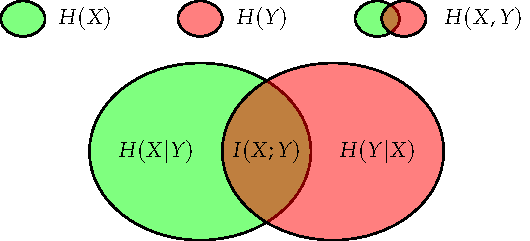
\includegraphics[width=0.8\textwidth]{Figures/information-theory/entropy-relations.pdf}
    \caption{熵和信息量的关系}
    \label{fig:entropy-relation}
\end{figure}

\section{Kullback-Leibler散度}\label{sec:kl-divergence}
\subsection{定义}
为了引入K-L散度,我们从互信息出发. 它的定义是:
\begin{align*}
    I(X;Y)&=H(X)-H(X|Y)\\
    &=-\sum_{x}p_X(x)\log p_X(x)+\sum_{x,y}p(x,y)\log\frac{p(x,y)}{p_Y(y)}\\
    &=-\sum_{x,y}p(x,y)\log p_X(x)+\sum_{x,y}p(x,y)\log\frac{p(x,y)}{p_Y(y)}\\
    &=\sum_{x,y}p(x,y)\log\frac{p(x,y)}{p_X(x)p_Y(y)}.
\end{align*}
根据\Cref{prop:information-doesnt-hurt},$I(X;Y)\geq 0$,等号成立当且仅当$X,Y$相互独立,即$p(x,y)=p_X(x)p_Y(y)$. $X,Y$之间的互信息越大,说明他们之间的关联越强,分布越不独立,$p(x,y)$越不接近$p_X(x)p_Y(y)$. 

上面的推导说明,互信息其实在用分布列的比值比较两个分布的接近程度,这样的想法可以被推广到一般分布上. 考虑两个概率分布的似然函数$p_1$和$p_2$(也就是他们的分布列). 抽取一个样本$X$,考虑如下两个假设:
\begin{center}
    $H_1$:样本$X$来自$p_1$的分布\quad vs.\quad $H_2$:样本$X$来自$p_2$的分布
\end{center}

为了判断哪个假设是更有可能的,我们考虑两个假设分布的似然比$p_1/p_2$. 如果这个比值越大,就越说明$p_1$的值更大,因而更有可能,倾向于接受$H_1$,反之则越倾向于接受$H_2$. 这种方法被称之为\emph{似然比检验法}.

从上述讨论出发,我们定义区分$H_1$和$H_2$的检验量为\emph{对数似然比}:
\[\log(p_1(x)/p_2(x)).\]
假设$H_1$是真的,那么在$H_1$成立的世界里,这个检验量的期望为
    \[\E_{X\sim p_1}(\log(p_1(X)/p_2(X)))=\sum_ip_1(i)\log\frac{p_1(i)}{p_2(i)}.\]
期望越大,说明$H_1$越有可能成立. 实际上,上面的期望就是K-L散度的定义.
\begin{definition}[Kullback-Leibler散度,相对熵]
    对于两个概率分布$p_1,p_2$,他们的\textbf{Kullback-Leibler散度}(\textbf{相对熵})定义为
    \[D_\KL(p_1\| p_2)=\E_{X\sim p_1}(\log(p_1(X)/p_2(X)))=\sum_ip_1(i)\log\frac{p_1(i)}{p_2(i)}.\]
其中规定$0\log(0/0)=0$,$0\log(0/a)=0$,$a\log(a/0)=+\infty$.
\end{definition}
我们马上知道,互信息是K-L散度的一种特殊情况:
\begin{proposition}\label{prop:mutual-information-kl-divergence}
    对于两个随机变量$X,Y$,成立$I(X;Y)=D_\KL(p_{X,Y}\|p_Xp_Y)$,其中$p_{X,Y}$是$X,Y$的联合分布列,$p_X,p_Y$分别是$X,Y$的边缘分布列.
\end{proposition}

K-L散度可以看成两个分布之间的区分衡量标准,但他不是度量. 一般来说,甚至连对称性都不成立. 例如,设$p_1$和$p_2$都是定义在$0,1$上的Bernoulli分布,参数分别为$1/2$和$1/4$. 于是
\[D_\KL(p_1\Vert p_2) = \frac12\log\frac{1/2}{3/4} + \frac12\log\frac{1/2}{1/4} = \frac12\log\frac43.\]
\[D_\KL(p_2\Vert p_1) = \frac34\log\frac{3/4}{1/2} + \frac14\log\frac{1/4}{1/2} = \frac12\log\frac{3\sqrt3}{4}.\]
这两个值是不相等的. 进一步,这个差值甚至可以到任意大(见习题\lhysays{出一下}).

上面推导K-L散度的过程看起来有些捏造,我们将在\Cref{sec:entropy-and-communication}中给出一个非常直观的理解方式. 现在,我们先接受这个定义,然后看一下K-L散度的一些性质.

\subsection{两个关于信息的不等式}
利用K-L散度,我们可以给出两个关于信息的不等式,它们分别是\emph{信息不等式}和\emph{数据处理不等式}.

\begin{theorem}[信息不等式]\label{thm:information-inequality}
    对于两个概率分布列$p,q$,成立$D_\KL(p\Vert q)\geq0$,当且仅当$p=q$时取等号.
\end{theorem}
\begin{proof}
    由于$\log x$是凸函数,所以由Jensen不等式,我们有
    \[D_\KL(p\Vert q)=-\E_{X\sim p}\left[\log\frac{q(X)}{p(X)}\right]\geq-\log \E_{X\sim p}\left[\frac{q(X)}{p(X)}\right]=-\log\sum_ip(i)\cdot\frac{q(i)}{p(i)}=0.\]
    因此,$D_\KL(p\Vert q)\geq0$,当且仅当$p=q$时取等号.
\end{proof}

信息不等式表明,K-L散度虽然不是度量,但却是非负的,因而确实可以被作为熵,用来衡量“额外的不确定性”. 此外,\Cref{prop:information-doesnt-hurt} 是信息不等式的直接推论. 利用类似的方法,我们可以证明条件互信息的非负性(即\Cref{prop:conditional-mutual-information} 中的第一条).

接下来我们叙述并证明数据处理不等式.
\begin{theorem}[数据处理不等式]\label{thm:data-processing-inequality}
    假设随机变量$X,Y,Z$形成了Markov链,那么$I(X;Y)\geq I(X;Z)$. 特别地,对任意函数$f$,成立$I(X;Y)\geq I(X;f(Y))$.
\end{theorem}
\begin{proof}
根据互信息链式法则,
    \begin{align*}
        I(X;Y,Z)&=I(X;Z)+I(X;Y|Z)\\
        &=I(X;Y)+I(X;Z|Y).
    \end{align*}
根据Markov性,条件在$Y$上,$X$和$Z$相互独立. 因此,$I(X;Z|Y)=0$,根据条件互信息的非负性,$I(X;Y|Z)\geq0$,所以$I(X;Y)\geq I(X;Z)$.

显然,$X,Y,f(Y)$也形成了Markov链,所以$I(X;Y)\geq I(X;f(Y))$.
\end{proof}

数据处理不等式表明,无论我们对随机变量$Y$进行了何种处理,甚至是允许带随机的处理,它的信息量都不会增加. 

\section{编码理论}\label{sec:entropy-and-communication}
最早的时候,Shannon建立信息论,就是为了给通信和编码理论一个数学基础. 从编码的角度出发,我们可以更本质地理解信息和熵. 

\subsection{熵与编码}

通信就是一个发射端和一个接收端,中间有信道传递消息. 将所有可能要传递的消息集合记为$\Omega$(一个有限集),我们现在考虑$\Omega$所蕴含的信息量是多少. 注意,根据Shannon的思想,$\Omega$里面具体是什么并不重要,重要的是有多少个. 我们可以用自然数$1,2,\dots$表示集合$\Omega$里的元素. 

使用二进制编码,我们至少需要$\log_2 |\Omega|$个比特来表示$\Omega$里的元素. 于是,假如说随机变量$X$表示收到的消息,那么$X$的\emph{熵}就定义为$H(X)=\log_2 |\Omega|$,它衡量了接收端收到的消息的不确定性. 

当我们选定了具体的消息$m\in \Omega$,$X$的不确定性被消除了,于是$X=a$的过程产生了(或者说传递了)$\log_2 |\Omega|$比特的信息. 比如说,我们发送一个长为 $n$ 的二进制序列,消息的集合大小就是$2^n$,发送任何一条具体的消息,我们就传递了 $n$ 比特的信息.

有时候,我们会把消息看成一个序列. 具体来说,我们可以发送独立的$k$条消息,其中第$i$条$X_i$来自消息集合$\Omega_i$,$|\Omega_i|=n_i$,那么$(X_1,\dots,X_k)$的熵就是
\[H(X_1,\dots,X_k)=\log_2 n_1+\dots+\log_2 n_k,\]
它衡量了$k$条消息的不确定性. 

在更常见的情况下,每次发送的其实不是一条消息,而是一个字母,所有的字母组成了一个字母表,我们用$\Sigma=\{x_1,\dots,x_s\}$来表示. 于是,$X_i$就是消息的第$i$个字母,于是,一条消息可以写作$X_1\dots X_k$,其中每一个$X_i$都来自$\Sigma$.

我们现在考虑更简单的情形,即每个字母$X_i$其实是同一个随机变量$X$的独立采样. 如果具体知道某一个$x_i$出现的次数,我们其实可以有更高效的传递信息的方式. 比如说,在极端情况下,如果只有$x_1$和$x_2$会出现,那么我们其实只需要$\log_2 2=1$比特就足够传递所有消息了:$0$表示$x_1$,$1$表示$x_2$.

在一般情况下,考虑$\Omega$中只包含长为$k$的消息,并且$x_i$在消息中出现$k_i$次,那么所有可能的消息数量为
\[|\Omega|=N(k)=\frac{k!}{k_1!\cdot\dots\cdot k_s!}.\]

假定我们需要$h(\omega)$比特来具体确定发的消息是$\omega$,我们来推导$h(\omega)$的上下界. 
\begin{itemize}
    \item 无论如何编码,我们需要能区分$\Omega$中的不同元素,这本身需要$\log_2\Omega$比特来表示. 
    \item 在一些编码中,我们还需要确定$(k_1,\dots,k_s)$. 确定它的一种方式是按照顺序给出每一个$k_i$. 因为$k_i\leq k$,每个$k_i$最多需要$\log_2 k$比特来表示,所以按顺序表示所有的$k_i$至多需要$s\log_2 k$比特.
\end{itemize}
于是,我们需要的比特数为
\[\log_2\frac{k!}{k_1!\cdot\dots\cdot k_s!}\leq h(m)\leq s\log_2k+\log\frac{k!}{k_1!\cdot\dots\cdot k_s!}.\]
这刚好和我们在统计力学中推导熵的过程是一致的!假设消息足够的长,$x_i$出现的频率逐渐接近$p_i$,那么同样的推理我们可以知道,
\[h(m)\sim -k\sum_i p_i\log_2 p_i=kH_2(p_1,\dots,p_s).\]
因此,如果知道字母的出现频率,我们传递单位长度的消息至少需要$H(p_1,\dots,p_s)$比特,这完全给出了熵的具体含义,而且,我们现在也不难理解熵的形式为何会出现$\log$了:熵就是期望上编码一个字母需要的比特数(即$\log(1/p(X))$).

那么,是否有一种编码确实达到了这个理论上的编码长度下界呢?答案是肯定的,它被称为\emph{Huffmann编码}. 它的核心思想在于把出现频率高的字母用更短的编码表示. 类似的思想被用在了机器学习的\emph{决策树}中,作为选择节点非常常用的一种依据.
\begin{remark}
    \emph{决策树}是一种常用的机器学习分类模型. 假设数据有很多属性$P_1,\dots,P_k$,这些属性共同决定了某一条数据的类别. 比如,在银行的信用系统中,给定了一个人的性别、是否已婚、是否负债等信息,我们希望给他评估一个信用评级. 
    
    决策树的做法是,将决策过程写成一棵树,然后叶节点是决策类别的结果. 比如说,我们会先看这个人是否负债,如果不负债,那么看是否已婚,如果已婚,那么我们信用评级就给A. 但如果负债,那么我们信用评级就给B. 
    
    那么,每个节点应该判断什么属性呢?树本身其实就是一种广义的消息,沿着树,从根节点走到叶节点得到的就是一条消息. 于是,在这一观点下,我们可以用熵与编码的关系来选择属性. 

    如果我们选择编码最短的属性,这样我们的决策树就会更加简单. 一种近似的做法是,对于每个节点,都优先选择信息增益最高的属性. 这样的选择方式叫做\emph{ID3策略}.
\end{remark}

我们进一步的问题是,为什么我们知道了每个字母的频次就可以压缩编码?我们接下来将要说明,其实长为$k$的消息中的“典型消息”的数量远远少于所有$k$长消息的数目,因此我们实际上相当于只是针对一个子集进行编码. 注意到,当$k$充分大的时候,
\[\log_2 N(k)\sim h(m)\sim kH_2(p_1,\dots,p_s).\]
因此,
\[N(k)\approx 2^{kH_2(p_1,\dots,p_s)}=\e^{kH(p_1,\dots,p_s)}.\]
然而,长为$k$的所有消息数目为
\[s^k=\e^{k\log s}.\]
根据\Cref{prop:entropy-maximum},只有当所有$p_i$相等的时候$N(k)$才会达到这一量级. 从这个意义上说,\emph{熵所刻画的信息量定量刻画了数据压缩可能的极限.}

以上关于信息编码下界以及数据压缩的讨论,再更一般的情况下也成立,此时这样的性质被称为\emph{渐近等分性}. 而这一性质成立对应的结果被称为\emph{Shannon–McMillan–Breiman定理},它的陈述以及证明都需要用到更多随机过程的知识,这里就不再给出了.

\subsection{K-L散度、交叉熵与编码}

我们在K-L散度的定义中提到了它的的另一个名字——相对熵. 实际上,这可以从编码中看出来. 假设事实上消息中字母的分布是$p_1$,那么期望上编码单位长度消息需要的比特数是
\[H(p_1)=\E_{X\sim p_1}[\log p_1(X)].\] 
如果我们错误地认为消息中字母的分布是$p_2$并使用最优编码,那么实际上期望编码单位长度消息需要的比特数是
\[\E_{X\sim p_1}[\log p_2(X)].\]
由于错误的认识所产生的额外编码长度是
\[\E_{X\sim p_1}[\log p_1(X)-\log p_2(X)]=D_\KL(p_1\Vert p_2).\]
根据本节中的讨论,我们知道,额外的编码长度代表的是额外的不确定性,因而这一概念是某种“熵”的概念. 这正是“相对熵”的由来,$D_\KL(p_1\Vert p_2)$表示了当我们错误地把$p_1$当成$p_2$时带来的额外的不确定性,或者说额外的信息损失.

在机器学习中,比起讨论K-L散度,更加常用的是直接讨论量$\E_{X\sim p_1}[\log p_2(X)]$. 从机器学习的观点来说,$p_1$是真实的分布,而$p_2$是我们所学习到的分布. 根据刚刚的讨论,这个量越小越说明$p_2$接近真实的$p_1$,因此这又是一种衡量两个分布之间关系的量,我们称之为\emph{交叉熵}:
\begin{definition}[交叉熵]
给两个随机变量$X,Y$,$X$的分布为$p_X$,$Y$的分布为$p_Y$,则$X$的分布$p_X$和$Y$的分布$p_Y$的\textbf{交叉熵}\footnote{文献中,经常会直接写为$H(p_X,p_Y)$,但是在本书中为了区分熵,我们使用了符号$CH$.}为
\[CH(p_X,p_Y)=-\E_{X\sim p_X}[\log p_Y(X)]=-\sum_ip_X(i)\log p_Y(i).\]
\end{definition}

在机器学习的分类问题中,我们希望学习到的分布$p_Y$尽可能地接近真实的分布$p_X$,所以我们训练的目标经常是最小化交叉熵$CH(p_X,p_Y)$. 有趣的是,从数理统计的角度来看,最小化交叉熵等价于进行\emph{最大似然估计}(见习题\lhysays{出一下}),因此这为最大似然估计提供了一种信息论意义下的理解.

\begin{remark}
现代的主流信息论都是从Shannon发展起来的. 然而,这一信息论也有很多问题. 
\begin{itemize}
    \item 信息论使用了概率论进行建模. 但我们已经看到,概率要么是作为频率的近似理论(频率学派),要么反映了人们对未知的信念(Bayes学派). 无论哪种解释,都将问题简化了. 正如Kolmogorov所说:“如果事情没有按照我们的预期发展,那么问题一定出在我们对于概率和真实世界的随机之间关系不清晰的认识上. ”
    \item 这一信息论考虑的是一族对象的信息. 我们是否能够用这样的方式来衡量单个对象的信息量呢?比如,我们要考虑这本书中包含的信息量,是它放在所有可能的书的集合中去考虑呢,还是把它的每一个章节分开考虑成一个随机序列呢?因此,信息论并不能很好地回答“单个对象”的信息量的问题. 
\end{itemize}

现代概率论的奠基人Kolmogorov也非常严肃地考虑了这一问题. 他提出了被后世称为\textbf{Kolmogorov复杂度}的概念,旨在刻画一个随机字符串的随机程度. 简单来说,一个字符串的Kolmogorov复杂度就是描述输出它所需要的最短代码长度. 越随机的字符串就越需要更复杂的程序去描述它的输出方式. 

例如,尽管字符串$x=0101010101$看起来非常长,但是我们可以用一个很短的程序来描述它:输出5次“$01$”. 然而,尽管字符串$y=011001$比$x$短得多,我们却很难找到一个简短的程序来描述它. 因此,$y$的Kolmogorov复杂度要比$x$大,因而看起来更像是随机的.

利用这一概念,我们可以将信息的概念变成一个对象自己的属性,而不再需要把对象放在可能的一堆对象中去考虑. 这是信息论的另一种构建思路. 
\end{remark}

\section{在机器学习中的应用:语言生成模型}\label{sec:language-models}
现如今,机器学习中最为瞩目的成果之一就是\emph{大语言模型}(LLM),它通过学习人类海量的高质量语料库来形成一个生成式的模型,其中最为典型的例子是ChatGPT.

从思路上来说,大语言模型的核心思想非常简单:给一段话,将其中一些词掩盖掉,让模型填出这些词来. 例如,给出
\begin{quotation}
    “我在\light{[mask]}面条,它真好吃. ”    
\end{quotation}
模型应该能够填出
\begin{quotation}
    “我在\light{吃}面条,它真好吃. ”
\end{quotation}

对于GPT模型来说,这一思想更加简单:永远只预测下一个词. 它的哲学是“通过预测下一个词,可以理解世界.”

这样的思想,对于更一般的数据也是成立的:用(修改过的)数据本身作为输入,训练一个\emph{编码器},然后将编码器的输出送入\emph{解码器},而解码器的输出具有原始数据的格式,我们希望这一输出能够尽量匹配原始的输入. 这正是本章开头Simon所说的“信息处理器”的具体实现. 

在语言模型中,一个\emph{生成模型}往往同时有编码器和解码器. 比如说,\Cref{fig:autoencoder} 展示的就是BART  \cite{lewisBARTDenoisingSequencetoSequence2019} 的结构.

\begin{figure}[ht]
    \centering
    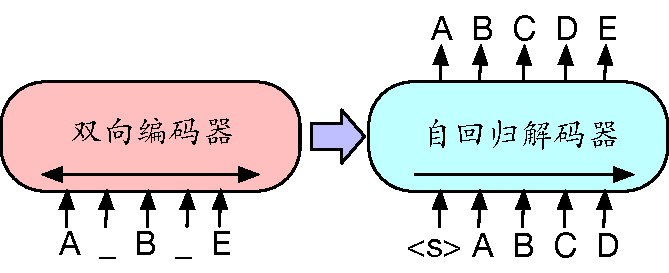
\includegraphics[width=0.65\textwidth]{Figures/information-theory/bart.pdf}
    \caption{生成式语言模型BART的示意图.}
    \label{fig:autoencoder}
\end{figure}

有的时候,编码器和解码器并不是显式给出的. 例如,GPT模型只有自回归解码器,没有编码器. 然而,我们可以认为GPT的解码器实际上是一个编码器-解码器的结构:它总要处理输入的数据,因而需要编码器,同时也要输出数据,因而需要解码器. 

在\Cref{sec:entropy-and-communication}我们指出,熵和编码有着密切的联系. 从这个角度出发,我们很容易理解生成模型背后的思想:我们希望通过训练的方式得到一个由神经网络所表示的编码和解码规则,他要尽可能符合真实数据的分布.

我们可以用一种非常简单的模型去理解这一过程. 假设所有的单词的集合为$\Sigma$,单词数为$k$的文本集合为$\Omega$. 我们希望训练一个生成模型$M$,给它输入$k-1$个单词,它可以给出第$k$个单词的概率分布,我们选择出现概率最大的那个词作为预测. 

在训练的时候,对于一个句子$\omega$,我们只保留前$k-1$个词,得到$\omega[1:k-1]$,然后将它输入到生成模型$M$中,让它去预测第$k$个词. 

对于这一个具体的句子$\omega$来说,理想的分布应该是一个\emph{Dirac分布}\footnote{Dirac分布是一个数学物理中更加常用的名字. 在概率论中,这也被称为\emph{退化分布};而在机器学习中,分布经常会表示为一个概率向量,文献中称为\emph{独热向量}. } $\delta_{\omega[k]}$,即以概率$1$取到$\omega[k]$. 假如说生成模型的输出是一个概率分布$M(\omega[1:k-1])=p$,那么,我们可以用K-L散度去衡量这两个分布的差异.

因为$H(\delta_{\omega[k]})$是固定的,所以我们只用考虑交叉熵$CH(\delta_{\omega[k]},p)$. 一次训练会给多个样本,所以我们的目标是同时最小化这些交叉熵的和. 假如训练集是$T$,我们的目标就是
\[
    \min_{M} \sum_{\omega\in T} CH(\delta_{\omega[k]},M(\omega[1:k-1])).
\]

实际上,这个例子是有普适性的,所有的监督训练的分类问题都可以用这种方式来建模. 而在\Cref{sec:decision-optimization-principle}我们也会看到,此时交叉熵实际上被作为了一种\emph{损失函数}.

\section{附录:Shannon定理的证明}\label{sec:Shannon-thm-proofs}
我们在这一部分给出Shannon定理(\Cref{thm:Shannon-thm})的证明. 整体上的思路是:
\begin{enumerate}
    \item 证明如果$f$是单调函数,对正整数$m,n$成立$f(mn)=f(m)+f(n)$,那么$f(n)=C\log n$.
    \item 求出$H(1/n,\dots,1/n)$的表达式.
    \item 假设$p_i$是有理数,设$p_i=n_i/\sum_j n_j$,考虑$\sum_j n_j$个等可能试验结果,利用假设3推出$H$的表达式.
    \item 利用有理数的稠密性和$H$的连续性推出一般情形.
\end{enumerate}
最后一步是显然的,我们只需要证明前三步即可.

对第一步,我们需要证明的是,如果$f$是单调函数,对正整数$m,n$成立$f(mn)=f(m)+f(n)$,那么$f(n)=C\log n$. 首先,利用数学归纳法容易看出,对正整数$n,k$,成立
\begin{equation}
    f(n^k)=kf(n).\label{eq:Shannon-thm-proof-1}
\end{equation}

设$m,n$是任意两个大于$1$的整数,再选任意大的正整数$k$,从$m$进制数的性质可以看出,总存在正整数$l$使得
\begin{equation}
    m^l\leq n^k < m^{l+1}.\label{eq:Shannon-thm-proof-2}
\end{equation}
根据$f$的单调性,我们有
\[
    f(m^l)\leq f(n^k) < f(m^{l+1}).
\]
利用式 \eqref{eq:Shannon-thm-proof-1},我们有
\[
    lf(m)\leq kf(n) < (l+1)f(m)\iff \frac{l}{k}\leq \frac{f(n)}{f(m)} < \frac{l+1}{k}.
\]
将式 \eqref{eq:Shannon-thm-proof-2} 取对数,得到
\[
    l\log m\leq k\log n < (l+1)\log m\iff \frac{l}{k}\leq \frac{\log n}{\log m} < \frac{l+1}{k}.
\]
所以
\[
    \left|\frac{\log n}{\log m}-\frac{f(n)}{f(m)}\right|\leq\frac1k.
\]
因为$k$可以是任意大的正整数,取$k\to\infty$,我们就得到了
\[
    \frac{\log n}{\log m}=\frac{f(n)}{f(m)}.
\]
由$m,n$的任意性,取$m=2$,我们就得到了$f(n)=(f(2)/\log 2)\cdot \log n= C\log n$. 容易检验,$f(1)=0=C\log 1$,因此这一等式对所有正整数$n$都成立.

对第二步,我们需要求出$f(n)=H(1/n,\dots,1/n)$的表达式. 我们要利用第一步的结果,首先,根据假设二,$f(n)$是单调递增的函数. 然后,考虑$mn$个等可能试验,我们可以将它分成两步试验,第一步有$m$中等可能的结果,而在每一种结果之下,第二步有$n$种等可能结果. 根据假设三,
\[
f(mn)=f(m)+\frac{1}{n}\cdot nf(n)=f(m)+f(n).    
\]
所以$f(n)$符合第一步的假设. 第二步就可以直接从第一步推出.

最后,我们证明第三步. 设$p_1,\dots,p_n$都是有理数,那么,他们可以被写为
\[
    p_i=\frac{n_i}{\sum_{j=1}^n n_j}.
\]
其中$n_i$是非负整数. 我们考虑$\sum_j n_j$个等可能试验,这个试验可以被看成两步的试验,第一步有$n$种可能的结果,第$i$种结果出现的概率是$p_i$,而在第$i$种结果之下,第二步有$n_i$种等可能的结果. 根据假设三,和证明的第三步,我们有
\[
   C\log\sum_{j=1}^nn_j=H(p_1+\dots+p_n)+\sum_{i=1}^n p_i\cdot C\log n_i.
\]
因此,
\begin{align*}
    H(p_1,\dots,p_n)&=C\left(\log\sum_{j=1}^nn_j-\sum_{i=1}^n p_i\log n_i\right)\\
    &=C\left(\log\sum_{j=1}^nn_j-\sum_{i=1}^n p_i\log\left(p_i\sum_{j=1}^n n_j\right)\right)\\
    &=C\left(\log\sum_{j=1}^nn_j-\sum_{i=1}^n p_i\log p_i-\sum_{i=1}^n p_i\log\sum_{j=1}^n n_j\right)\\
    &=-C\sum_{i=1}^n p_i\log p_i.
\end{align*}
这正是我们要证明的. 于是,我们证明了Shannon定理.

\section{习题}
\begin{enumerate}[wide, labelindent=0pt]
    \item 我们在熵以及K-L散度的定义中,都规定了一些无定义的量的值,这些值并不是随便规定的,他们实际上反映了熵或者K-L散度定义中的连续性.
    \begin{enumerate}
        \item 证明:对给定的$a>0$,$\lim_{x\to 0+}x\log (x/a)=0$,因此我们规定了$0\log 0=0$以及$0\log(0/a)=0$.
        \item 证明:对给定的$a>0$,$\lim_{x\to 0+}x\log (a/x)=+\infty$,因此我们规定了$0\log(a/0)=+\infty$.
    \end{enumerate}
    
    \item 考虑关于$n$的正实数序列$a_1(n),\dots,a_k(n)$以及$b_1(n),\dots,b_k(n)$,假设对所有$i$,都成立$\lim_{n\to\infty} a_i(n)/b_i(n)=1$,证明:
    \[\lim_{n\to\infty}\frac{a_1(n)+\dots+a_k(n)}{b_1(n)+\dots+b_k(n)}=1.\]
    由此证明式 \eqref{eq:logP}.
    
    \item 证明\Cref{prop:entropy-2prob}.
    
    \item 用Lagrange乘子法重新证明\Cref{prop:entropy-maximum}.
    \begin{hint}
        如果你不知道Lagrange乘子法,可以参考 \Cref{???}.
    \end{hint}

    \item 证明\Cref{prop:conditional-mutual-information}.
    
    \item \cite{tingAmountInformation1962a} 仿照集合论的思路,我们可以定义三个随机变量的互信息为:
    \[I(X;Y;Z)=I(X;Y)-I(X;Y|Z).\]
    \begin{enumerate}
        \item 证明对称性:$I(X;Y;Z)=I(Y;X;Z) = I(X;Z;Y)$.
        \item 举一个例子说明,可能会有$I(X;Y;Z)<0$,所以这样定义的互信息并不一定真的代表“信息量”.
    \end{enumerate}

    \item 举一个例子说明,即便$D_\KL(p_1\Vert p_2)$很接近$0$,$D_\KL(p_2\Vert p_1)$也可能会很大.
    
    \item (\emph{单变量数据处理不等式})对任意离散随机变量$X$和函数$f$,证明:$H(X)\geq H(f(X))$.

    \item 考虑二分类的学习问题,此时对单个样本我们观察到的结果要么是$0$或$1$,假设在真实世界中样本总体服从参数为$\theta$的Bernoulli分布,即$\Pr(X=1)=1-\Pr(X=0)=\theta$. 假设我们的数据集是$(x_1,y_1),\dots,(x_N,y_N)$,他们是从总体中独立采样得到的. 
    \begin{enumerate}
        \item 将问题考虑成一个数理统计问题,估计$\theta$. 写出似然函数$L(\theta;y_1,\dots,y_N)$.
        \item 再将问题考虑为一个信息论问题,写出每个样本的真实分布与估计分布之间的交叉熵之和$CH(\theta;y_1,\dots,y_N)$.
        \item 证明:$\max_{\theta} L(\theta;y_1,\dots,y_N)=\min_{\theta} CH(\theta;y_1,\dots,y_N)$,也就是说,\emph{最大似然估计等价于最小化交叉熵}.
    \end{enumerate}

    \item 请查找文献回答以下问题:
    \begin{enumerate}
        \item Fisher信息量是什么?它与K-L散度有什么样的关系?
        \item 列举其他概率分布之间散度的概念,他们是否是度量?
        \item 列举概率分布之间的度量,他们之间是否有关联?
    \end{enumerate}
    
\end{enumerate}
\section{章末注记}
信息一词的英文是“information”,从动词“inform”来,意思是告知、通知. 早在15世纪中叶,“information”一词的出现了义项“在通信中针对特定主题的知识”.\cite{InformationEtymologyOrigin} 这说明在那个时候人类就已经意识到,通信会产生新的东西,被称为知识或信息. 然而,人类对信息的严谨探索起步晚得多. 关于信息的物理学讨论源自统计力学,Boltzmann提出了著名的熵,证明了H定理,以此给出了热力学第二定律的微观解释. 关于Boltzmann的工作,参见 \cite{uffinkBoltzmannWorkStatistical2022}. 

一般认为,现代信息论的起源是Shannon的论文 \cite{shannonMathematicalTheoryCommunication1948},他在论文中提出了信息的数学定义,以及信息的基本性质. 但是,Shannon的工作并不是孤立的,他的工作是在统计力学的基础上发展起来的. 事实上,Shannon在论文中也提到了Boltzmann的熵. 这篇工作也被视为通信理论以及编码理论的奠基性工作.  Shannon在这篇论文中还给出了渐近意义下达到理论下界的最优编码,并且独立地被Fano \cite{robertm.fanoTransmissionInformation1949} 以一种不同的形式发现,因此后世称为Shannon-Fano编码. 但是Shannon-Fano编码并不是精确地达到下界,实际上,最优编码是Huffman \cite{huffmanMethodConstructionMinimumRedundancy1952} 给出的. Shannon在这篇论文中还讨论了渐近等分性,后来MciMillan的工作 \cite{mcmillanBasicTheoremsInformation1953} 和 Breiman的工作 \cite{breimanIndividualErgodicTheorem1957} 拓展了这一结果,因此后世称为Shannon-McMillan-Breiman定理. 

关于信息论与集合论的关系工作,可以参见Hu Kuo Ting的工作 \cite{tingAmountInformation1962a}. 他的工作还给出了多个随机变量互信息的定义,在这一章习题中有涉及.

相对熵的概念依然是从Shannon的奠基性论文 \cite{shannonMathematicalTheoryCommunication1948} 中提出的,但他只局限于通信的问题. 更加一般的讨论是由Kullback和Leibler在 \cite{kullbackInformationSufficiency1951} 给出,他们的是一种数理统计的思路,但是他们也具体地讨论了这一概念与信息的关系. 他们的论文中也讨论了交叉熵这一概念. 

机器学习中编码器和解码器的思路,最早是由Rumelhart,Hinton和Williams在 \cite{rumelhartLearningInternalRepresentations1986} 中提出,他们将编码器和解码器的整体称作\emph{自编码器}. 这篇工作几乎可以被视为深度学习的开山之作,它还提出了训练神经网络最常用的反向传播算法.

关于信息论的经典教科书,可以参见 \cite{coverElementsInformationTheory2012} ,此外,概率论的教材中也有很多很好的讨论,比如 \cite{jaynesProbabilityTheoryLogic2002},\cite{shiryaevProbability1996} 以及\cite{LiXianPingGaiLuLunJiChu2010}.

关于Kolmogorov复杂度的讨论,可以参见专著 \cite{???},这本书对于随机、信息、编码、复杂度,乃至归纳推理等概念都有非常独到的见解,值得一读. 